\documentclass[pdflatex,sn-mathphys-num]{sn-jnl}

\usepackage{graphicx}
\usepackage{listings}
\usepackage{xcolor}
\usepackage{booktabs}
\usepackage{float}
\usepackage{caption}
\usepackage{subcaption}
\usepackage{amsmath}
\usepackage{tcolorbox}
\usepackage{lipsum}
\usepackage{multirow}
\usepackage{mathrsfs}
\usepackage{amssymb}
\usepackage{algorithm}
\usepackage{algpseudocode}

\newtcolorbox{promptbox}{
  colback=gray!15,
  colframe=black,
  boxrule=0.5pt,
  arc=0pt,
  left=3pt, right=3pt,
  top=3pt, bottom=3pt,
  fontupper=\small
}

\begin{document}

\title{RL Market Maker — Feature Engineering for Linear Function Approximation (VFA)}

\author*[1]{\fnm{Carlo} \sur{Falchi}}\email{cfalchi@gmail.com}

\affil[1]{\orgdiv{Department of Computer Science}, \orgname{University of Milan}, \country{Italy}}

\abstract{
This project investigates the application of reinforcement learning for portfolio management and 
market-making in a financial environment characterized by stochastic price dynamics and regime switches. 
We focus on the interplay between feature engineering and learning performance under Linear Value Function Approximation (VFA).
We evaluate a semi-gradient SARSA agent using three distinct feature sets---raw prices, asset allocations, and technical indicators---paired 
with four basis-function architectures: raw linear representation, tile coding, radial basis functions (RBF), and degree-2 polynomial expansions. 
Our results demonstrate that the choice of feature map critically determines learning success. 
Global approximation methods, such as raw and polynomial features, consistently fail by either diverging or collapsing into degenerate single-action policies. 
Conversely, local and sparse generalization via tile coding stabilizes the semi-gradient updates and achieves the best overall performance, while RBF networks produce comparable returns but with higher variance. 
Finally, we discuss the inherent representational limitations and projection-error floor of linear VFA in noisy, partially observable market environments, motivating a transition to deep reinforcement learning methods like Deep Q-Networks (DQN).
}

\maketitle

\section{Introduction}
This project uses reinforcement learning (RL) to design market-making and portfolio management agents 
for financial markets using high-frequency historical equities data. 
It is primarily focused on the interplay between feature engineering and learning performance 
in the context of Linear Function Approximation (LFA). 
We analyze and compare different feature sets and basis function architectures. 

Market making and portfolio control have been studied across a number of disciplines, 
including economics, quantitative finance, artificial intelligence, and machine learning. 
A classic approach in the finance literature treats market making as a problem of stochastic optimal control.

In this work, we train a semi-gradient SARSA agent with linear function approximation on three sets of state features 
--- raw prices, portfolio allocations, and hand-crafted technical indicators (RSI, MACD, rolling volatility) --- 
each paired with four basis-function architectures: raw linear, tile coding, radial basis functions (RBF), and degree-2 polynomial expansions. 

\section{Problem Description}
\label{sec:problem}

The agent manages a small portfolio of assets over a finite time horizon. At each time step, it observes a set of market and portfolio signals and decides how to allocate its capital across a discrete set of joint trading actions (e.g., buy, hold, or sell for each asset). Prices evolve according to a hidden stochastic process featuring regime switches, requiring the agent to adapt its policy over time. The reward at each step reflects the relative return on portfolio wealth. The market occasionally transitions into a crisis regime in which asset correlations shift sharply and volatility spikes.

\section{Dataset and Price Dynamics}
\label{sec:data}

To calibrate the parameters of the stochastic price distributions, daily historical asset prices were collected from Yahoo Finance spanning July 2019 to July 2026. The asset universe represents a multi-asset allocation strategy comprising equities, fixed income, and cryptocurrencies:
\begin{itemize}
    \item \textbf{Global Equities ETF}: VWCE (Vanguard FTSE All-World UCITS ETF)
    \item \textbf{Bonds ETF}: C3M (Amundi Short-Term Euro Government Bond ETF)
    \item \textbf{Cryptocurrency}: BTC (Bitcoin)
\end{itemize}

\subsection{Price Dynamics Model}
To simulate market behavior under stochastic settings, asset prices are modeled using a Multivariate Geometric Brownian Motion (GBM) in discrete time. The continuous price vector $\mathbf{S}(t)$ follows:
\begin{equation}
    d\mathbf{S}(t) = \operatorname{diag}(\mathbf{S}(t)) \left( \boldsymbol{\mu} dt + \mathbf{\Sigma}^{1/2} d\mathbf{W}(t) \right)
\end{equation}
where $\boldsymbol{\mu}$ and $\mathbf{\Sigma}$ represent the continuous-time drift vector and return covariance matrix, respectively. Integrating over a single discrete time step $\Delta t = 1$ yields the exact transition equation:
\begin{equation}
    \mathbf{S}_{t+1} = \mathbf{S}_t \odot \exp(\mathbf{r}_t), \quad \text{where } \mathbf{r}_t \sim \mathcal{N}(\boldsymbol{\mu}_k, \mathbf{\Sigma}_k)
\end{equation}
Here, $\odot$ denotes Hadamard (element-wise) multiplication, and the distribution parameters $(\boldsymbol{\mu}_k, \mathbf{\Sigma}_k)$ shift according to the active market regime $k \in \{\text{Normal}, \text{Crisis}\}$ calibrated directly from empirical historical returns.

\section{Market Environment POMDP}
\label{sec:pomdp}

We model the portfolio management problem as a Partially Observable Markov Decision Process (POMDP). The state representation is partially observable with respect to the active market regime $k \in \{\text{Normal}, \text{Crisis}\}$. Technical features—such as RSI \cite{wilder1978new}, rolling volatility, MACD \cite{appel2005technical}, and average correlation—serve as the observable signals from which the hidden regime can be implicitly inferred, rendering feature design central to policy performance.

\subsection{State Space}
The state $\mathcal{S}$ is represented by the vector $s \in \mathbb{R}^{11}$ which concatenates market signals and portfolio internal features:
\begin{itemize}
    \item $\mathbb{R}_+^N$: Current asset prices ($N = 3$)
    \item $[0,1]^N$: Portfolio allocation per asset (fraction of total portfolio wealth)
    \item $[0,1]$: Cash ratio
    \item $[0,100]$: Relative Strength Index (RSI) \cite{wilder1978new} of portfolio wealth ($14$-step window)
    \item $[-1,1]$: Average pairwise return correlation across assets ($20$-step window)
    \item $\mathbb{R}_+$: Rolling portfolio return standard deviation / volatility ($20$-step window)
    \item $\mathbb{R}$: MACD \cite{appel2005technical} histogram of portfolio wealth, normalized by total wealth
\end{itemize}
While prices, allocations, and cash ratio capture position state, the remaining indicators provide engineered risk signals.
More details about the features are in Section \ref{sec:pomdp}.
\subsection{Action Space}
We model the action space as a MultiDiscrete space $\mathcal{A} = \{0, 1, 2\}^N$, where $N = 3$ is the number of risky assets. An action $\mathbf{a} = (a_1, \dots, a_N) \in \mathcal{A}$ directly specifies the operation to execute on each asset $i$:

\begin{equation}
    a_i = 
    \begin{cases}
        0, & \text{\textbf{Sell}: Liquidate $10\%$ of holdings in asset } i \text{ (subject to fee rate } \eta = 0.10\text{)} \\
        1, & \text{\textbf{Hold}: Maintain current position in asset } i \\
        2, & \text{\textbf{Buy}: Allocate $10\%$ of available cash to purchase asset } i
    \end{cases}
\end{equation}

\subsection{Environment Step Dynamics}
At time step $t$, given current prices $\mathbf{p}_t = [p_{1,t}, \dots, p_{N,t}]^T$, cash $C_t$, and share holdings $\mathbf{h}_t = [h_{1,t}, \dots, h_{N,t}]^T$, executing the multi-discrete action vector $\mathbf{a}_t = (a_{1,t}, \dots, a_{N,t}) \in \{0, 1, 2\}^N$ transitions the environment through three phases:

\begin{enumerate}
    \item \textbf{Trade Execution}: For each asset $i \in \{1, \dots, N\}$, the corresponding trading operation $a_{i,t}$ is executed sequentially:
    \begin{itemize}
        \item \textit{Sell ($a_{i,t} = 0$)}: Liquidate $\Delta h_i = 0.10 \cdot h_{i,t}$ shares. Cash increases after applying a penalty fee rate $\eta = 0.10$:
        \begin{equation}
            C_t \leftarrow C_t + (1 - \eta) \cdot \Delta h_i \cdot p_{i,t}, \quad h_{i,t} \leftarrow h_{i,t} - \Delta h_i
        \end{equation}
        \item \textit{Hold ($a_{i,t} = 1$)}: Share holdings $h_{i,t}$ remain unchanged.
        \item \textit{Buy ($a_{i,t} = 2$)}: Allocate cash $B_i = 0.10 \cdot C_t$ to purchase $\Delta h_i = B_i / p_{i,t}$ shares:
        \begin{equation}
            C_t \leftarrow C_t - B_i, \quad h_{i,t} \leftarrow h_{i,t} + \Delta h_i
        \end{equation}
    \end{itemize}
    
    \item \textbf{Market \& Regime Transition}: The market environment advances to step $t+1$:
    \begin{itemize}
        \item \textit{Regime Transition}: The market regime $k_{t+1} \in \{0, 1\}$ evolves according to a two-state Markov chain parameterized by persistence probabilities $p_{\text{stay, normal}}$ and $p_{\text{stay, crisis}}$.
        \item \textit{Price Step}: Under stochastic simulation, asset prices transition via Geometric Brownian Motion: $p_{i,t+1} = p_{i,t} \cdot \exp(r_{i,t})$, where $\mathbf{r}_t \sim \mathcal{N}(\boldsymbol{\mu}_{k_{t+1}}, \mathbf{\Sigma}_{k_{t+1}})$.
    \end{itemize}
    
    \item \textbf{State Evaluation}: Updated total portfolio wealth is evaluated as $W_{t+1} = C_t + \sum_{i=1}^N h_{i,t} \cdot p_{i,t+1}$. The environment emits step reward $r_{t+1}$, updated observation vector $s_{t+1}$, and sets termination $\text{terminated} = \text{True}$ if bankruptcy occurs ($W_{t+1} \le 0$).
\end{enumerate}

\subsection{Reward Function}
The reward $r_t \in \mathbb{R}$ at step $t$ measures the simple relative return on total portfolio wealth $W_t$:

    $$r_t = \dfrac{W_t - W_{t-1}}{W_{t-1}}$$
        
    

where $\displaystyle W_t = C_t + \sum_{i=1}^N h_{i,t} \cdot p_{i,t}$ represents total wealth.

\subsection{Discount Factor and Horizon}
We set the discount factor to $\gamma = 1.0$. Episodes are capped at a maximum of $250$ time steps, treating truncation as terminal, ensuring that the undiscounted episodic return remains well-defined.

\subsection{Experimental Environment Configuration}
Unless stated otherwise, all empirical evaluations are conducted under a stochastic environment subject to regime-switching dynamics. The default environment settings are detailed in Table~\ref{tab:env_params}.

\begin{table}[h!]
\centering
\caption{Baseline Environment Hyperparameters and Technical Indicator Settings}
\label{tab:env_params}
\begin{tabular}{lll}
\hline
\textbf{Parameter} & \textbf{Symbol / Variable} & \textbf{Default Value} \\ \hline
\multicolumn{3}{l}{\textit{Environment \& Capital Settings}} \\
Initial Portfolio Wealth & $W_0$ & $\$10{,}000.00$ \\
Stochastic Simulation & -- & \texttt{True} \\
Regime-Switching Dynamics & -- & \texttt{True} \\ \hline
\multicolumn{3}{l}{\textit{Regime Transition Parameters}} \\
Normal Regime Persistence Probability & $p_{\text{stay, normal}}$ & $0.97$ \\
Crisis Regime Persistence Probability & $p_{\text{stay, crisis}}$ & $0.85$ \\
Crisis Drift Scaling Factor & $\alpha_{\mu}$ (\texttt{crisis\_mu\_scale}) & $-2.0$ \\
Crisis Covariance Scaling Factor & $\alpha_{\Sigma}$ (\texttt{crisis\_cov\_scale}) & $3.0$ \\ \hline
\multicolumn{3}{l}{\textit{Technical Indicator Windows}} \\
RSI Lookback Window & $W_{\text{RSI}}$ & $14$ steps \\
Correlation Lookback Window & $W_{\text{corr}}$ & $20$ steps \\
Volatility Lookback Window & $W_{\text{vol}}$ & $20$ steps \\
MACD Fast EMA Span & $K_{\text{fast}}$ & $12$ steps \\
MACD Slow EMA Span & $K_{\text{slow}}$ & $26$ steps \\
MACD Signal Line Span & $K_{\text{signal}}$ & $9$ steps \\ \hline
\end{tabular}
\end{table}

\section{Discretization Problem}
\label{sec:discretisation}

All features in our Market Environment have continuous values. 
While discretizing these features constructs a finite state space to which tabular Q-learning could be applied, 
it transforms the fully observable continuous MDP into a Partially Observable Markov Decision Process (POMDP). 
Because the agent observes only a bin index, many distinct continuous states are aliased onto the same discrete observation. 
Consequently, the Markov property fails on the agent's observations, Q-learning's convergence guarantees no longer apply to the underlying optimal value function, 
and structural noise is introduced into the agent's transitions. 
This severe limitation of tabular discretization in continuous domains motivates our adoption of Value Function Approximation.

\section{Value Function Approximation}
\label{sec:vfa}

The Value Function Approximation is the family of methods that represents
$Q$ (action-value function) as a parametric function $\hat{q}(s,a,\mathbf{w})$
rather than a table, where in the linear case $$Q(s, a; \mathbf{w}) = \mathbf{w}^\top \mathbf{x}(s)$$

Where: 
\begin{itemize}
    \item $s$ is the state and $a$ is the chosen action.
    \item $\mathbf{x}(s)$ is the feature vector extracted from state $s$.  
    \item $\mathbf{w} \in \mathbb{R}^d$ is the weight vector corresponding to action $a$. With $d$ much smaller than $|S| \times |A|$  
\end{itemize}

The structural payoff is generalization, if the parametric family is well chosen, "states whose features overlap" coincides with "similar states", and the algorithm automatically does what tabular methods could not, it transfers knowledge from one state to its neighbours.
On the other side parameter update that improves the value estimate at one state may worsen it at another state with overlapping features.

In the function approximation setting, the agent's update becomes a gradient-based adjustment of the parameter vector that induces a change at the state of interest and a residual change everywhere else.
\subsection{Linear FA SARSA Agent \& Semi Gradient}
For Episodic Semi-Gradient Sarsa, the target $y_t$ is defined as the 1-step TD target using the next state-action pair:$$y_t = r_{t+1} + \gamma \, \hat{q}(S_{t+1}, A_{t+1}; \mathbf{w})$$

The true gradient is: $$\nabla_{\mathbf{w}} \mathcal{L}_t = - \left[ y_t - \hat{q}(S_t, A_t; \mathbf{w}) \right] \left[ \nabla_{\mathbf{w}} \hat{q}(S_t, A_t; \mathbf{w}) - \gamma \nabla_{\mathbf{w}} \hat{q}(S_{t+1}, A_{t+1}; \mathbf{w}) \right]$$
Substituting $y_t$ into the semi-gradient update rule yields:$$\mathbf{w} \leftarrow \mathbf{w} + \alpha \left[ r_{t+1} + \gamma \, \hat{q}(S_{t+1}, A_{t+1}; \mathbf{w}) - \hat{q}(S_t, A_t; \mathbf{w}) \right] \nabla_{\mathbf{w}} \hat{q}(S_t, A_t; \mathbf{w})$$
This differs from the true gradient by the drop of the second term and $\nabla_{\mathbf{w}} \hat{q}(S_t, A_t; \mathbf{w}) = \mathbf{x}(s)$

The term is dropped for three reasons:
\begin{itemize}
\item Computational simplicity: only scale and add a single feature vector
\item Empirical effectiveness: The bias introduced by ignoring the target's dependence on $\mathbf{w}$
 is typically modest and the resulting updates have the same direction as the tabular update
\item Conceptual fidelity to the bootstrap idea: the whole point of bootstrapping is to use the current estimate at $S_{t+1}$
 as a fixed reference for improving the estimate at $S_t$, target is a function of the parameters that we are jointly optimizing 
 so adjusting it would defeat the purpose.

The semi-gradient is a fixed-point iteration but not the minimum of any loss (SGD assume a fixed loss landscape), so the convergence guarantees of gradient descent do not apply.
In the linear case, on-policy (like SARSA) semi-gradient TD converges; off-policy semi-gradient TD, can fail to converge, and even diverge.
Second the target moves as $\mathbf{w}$ changes. Updates that improve the prediction at one state can shift the target at neighbouring states, requiring further updates.
\end{itemize}

\section{Feature Map}
\label{sec:featuremap}

The feature vector $\mathbf{x}(s) \in \mathbb{R}^d$ is not learned. Different feature maps produce different generalization patterns:
tile coding and radial basis functions generalize locally; polynomial features generalize globally; price-only features generalize linearly along each axis.

A tabular Q-table can represent any function on a finite state space exactly.
The best the approximator can do is the projection of $q^{\pi}$ (optimal) onto the representable space,
which depends on the features, on the on-policy distribution, and on the geometry of the feature map. 
This projection error is a property of the representation, not a learning artefact, and no amount of additional training reduces it.

The essential trick of linear function approximation is that we move the non-linearity into the features, while keeping the model linear in the weights. 
The feature map  can be as non-linear as we want and the resulting 
$\mathbf{w}^\top \mathbf{x}(s)$ inherits all of that non-linearity in $s$.

Figure \ref{fig:featureRepresentation} shows the different representations of two features, MACD and Volatility, using the three different feature maps: Tiling, RBF, and Polynomial.

\begin{figure}[ht]
    \centering
    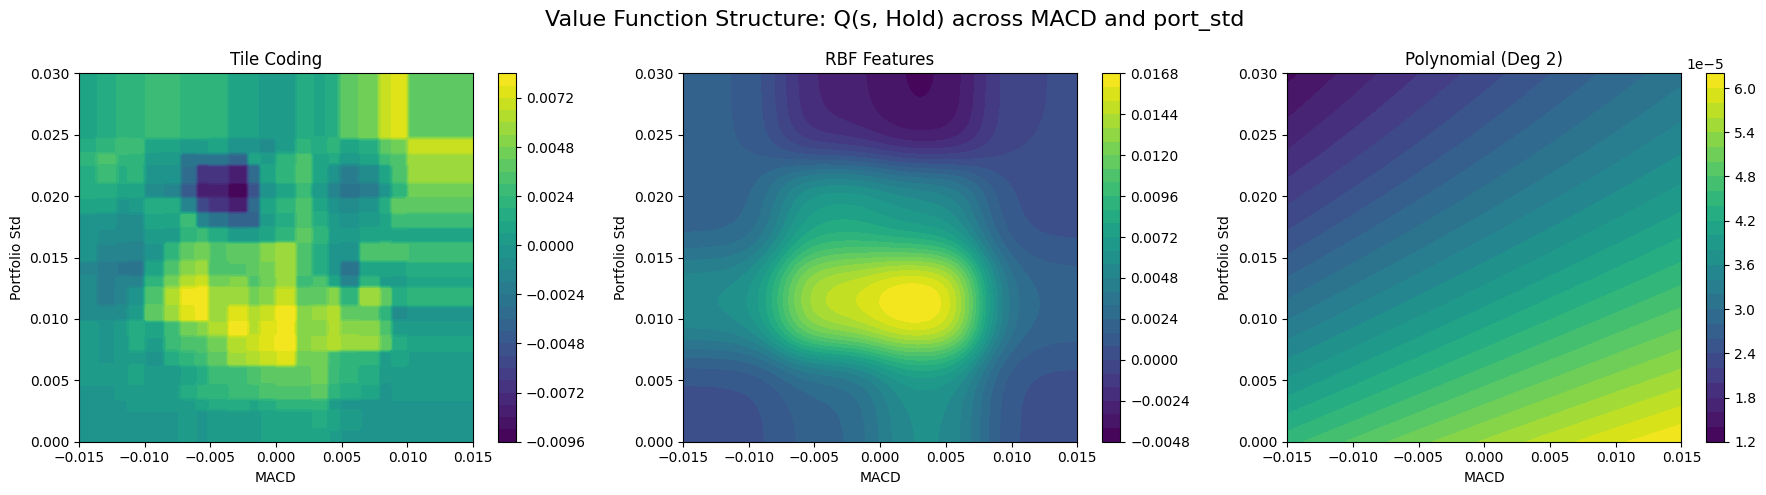
\includegraphics[width=0.9\textwidth]{charts/feature_representation.png}
    \caption{Representation of MACD and Volatility}
     \label{fig:featureRepresentation}
\end{figure}

\subsection{Raw Feature Representation}

The simplest baseline mapping uses the raw continuous state components directly as the feature vector $\mathbf{x}(\mathbf{s}) = \mathbf{s}$ without non-linear transformation or expansion. This mapping constrains the estimated action-value surface to be an affine hyperplane over the state space. Because hyperplanes cannot capture non-linear market patterns or state interactions, raw features often serve primarily as a baseline to highlight the necessity of richer basis functions.

\subsection{Tile Coding Representation}

Tile coding maps a continuous state vector $\mathbf{s} \in \mathcal{S}$ into a sparse binary feature vector $\mathbf{x}(\mathbf{s}) \in \{0, 1\}^{d}$. For a state space bounded by $[\mathbf{s}_{\text{low}}, \mathbf{s}_{\text{high}}]$, the state space is partitioned using $T$ distinct, overlapping tilings grid structures. Because exactly one tile is active per tiling at any given state $\mathbf{s}$, the representation is sparse, containing exactly $T$ non-zero elements, enabling locally-generalizing linear updates.

\subsection{Radial Basis Functions (RBF)}

Radial Basis Functions (RBFs) provide a smooth, dense, non-linear feature representation by evaluating the similarity of a state $\mathbf{s}$ to a set of fixed points (centers) $\mathbf{c}_i$ evenly distributed across the state space. For each feature, the activation is computed via a Gaussian function with bandwidth parameter $\sigma$. Unlike tile coding, RBF representations are dense, producing non-zero activations across the grid, allowing for smooth, differentiable value function estimates.

\subsection{Polynomial Basis Functions}

Polynomial feature extraction models non-linear interactions by generating cross-terms and squared terms up to a specified maximum degree (we set $p = 2$). This allows a linear weight update to capture non-linear relationships among state variables. To avoid numerical instability, state features are first normalized from their original bounds to $[-1, 1]$.

\subsection{Feature Configurations Summary}

The exact state components, grid resolutions (or centers), and resulting feature dimensionalities for each evaluated configuration are summarized in Table~\ref{tab:feature_configs}.

\begin{table}[htbp]
\centering
\caption{Feature map configurations across different feature sets.}
\label{tab:feature_configs}
\begin{tabular}{lllcc}
\toprule
\textbf{Feature Map} & \textbf{Set} & \textbf{State Features} & \textbf{Resolution / Degree} & \textbf{Dim. ($\mathbf{x}$)} \\
\midrule
Raw & Set A & Raw Asset Prices & -- & 3 \\
\midrule
Tile Coding ($T=4$) & Set A & Raw Asset Prices & $[5, 5, 5]$ grids & 500 \\
& Set B & Asset Allocations, Cash & $[5, 5, 5, 5]$ grids & 2,500 \\
& Set C & MACD, Vol., RSI & $[4, 5, 4]$ grids & 320 \\
\midrule
RBF ($\sigma=0.1$) & Set C & MACD, Vol., RSI & $[4, 4, 4]$ centers & 64 \\
\midrule
Polynomial ($p=2$) & Set B & Asset Allocation, Cash & $D=4$ inputs & 15 \\
& Set C & MACD, Vol., RSI & $D=3$ inputs & 10 \\
\bottomrule
\end{tabular}
\end{table}
\section{Training \& Evaluation}
\label{sec:training}

A single training episode follows a fixed pattern, repeated until termination or truncation.

At every step:
\begin{itemize}
    \item The agent picks an action using its current behavior policy, which is $\epsilon$-greedy with respect to the current estimated Q-values.
    \item The environment executes the action, advancing one transition.
    \item The agent updates the weights $\mathbf{w}$ using the semi-gradient from the realized transition, passing even the next action $A_{t+1}$ based on the new observed state $S_{t+1}$ (SARSA).
\end{itemize}

In our POMDP Market environment, which has a finite horizon, the episode ends after 250 steps or if the portfolio value goes to 0.
At that point, the agent runs the $\epsilon$ decay (beginning with $\epsilon$ fixed to $1.0$ for more exploration, then gradually decaying by a factor of $0.997$ for more exploitation). 
With this configuration of $\epsilon$-decay, the agent will achieve the minimum exploration rate after 997 episodes, with $\epsilon_{\min}$ fixed to $0.05$.
\begin{table}[htbp]
\centering
\caption{Hyperparameter}
\label{tab:hyperparameters}
\begin{tabular}{ll}
\hline
\textbf{Parameter} & \textbf{Value} \\ 
\hline
\multicolumn{2}{l}{\textit{Training Schedule}} \\
Number of Episodes & $2000$ \\
Evaluation Frequency& $50$ \\
Evaluation Episodes  & $20$ \\
Max Steps per Episode - Train  & $250$ \\
Max Steps per Episode - Eval & $250$ \\
\hline
\multicolumn{2}{l}{\textit{Agent \& Exploration}} \\
Discount Factor ($\gamma$) & $1.0$ \\
Initial Exploration Rate ($\epsilon_{\text{start}}$) & $1.0$ \\
Minimum Exploration Rate ($\epsilon_{\text{min}}$) & $0.05$ \\
Exploration Decay Rate ($\epsilon_{\text{decay}}$) & $0.997$ \\
Initial Weight Value ($w_{\text{init}}$) & $0.0$ \\
\hline
\end{tabular}
\end{table}
\subsection{Tracking}
For every episode we store the episode return (the sum of rewards collected), and the episode length (number of steps).
\begin{itemize}
\item \textbf{Training Return}: The episode returns collected during training are produced by the $\epsilon$-greedy behavior policy (learning \& exploring).
\item \textbf{Greedy Evaluation}: The episode returns obtained when the agent acts greedily (no exploration). We run a small batch of evaluation episodes every $50$ training episodes to track learning progress.
\item \textbf{Weight Norm}: To monitor parameter health $\mathbf{w}$, we use the Frobenius norm $\|\boldsymbol{W}\|_F = \sqrt{\sum_{a,i} W_{a,i}^2}$ where $\boldsymbol{W}$ is a matrix of weight features. In a stable regime, this converges to a finite value (plateau).
\end{itemize}
\section{Results}
\label{sec:results}

For every feature configuration, we repeat the training with 3 different seeds to assess the standard deviation 
and the stability of the learned policy. 
Table~\ref{tab:final_results} summarizes the final greedy evaluation returns after $2000$ training episodes, together with the final weight norm.

\begin{table}[htbp]
\centering
\caption{Final greedy evaluation return (mean $\pm$ std over 3 seeds) and final weight norm after $2000$ training episodes}
\label{tab:final_results}
\begin{tabular}{lllccc}
\toprule
\textbf{Set} & \textbf{State Features} & \textbf{Map} & $d$ & \textbf{Eval Return} & $\|\mathbf{W}\|_F$ \\
\midrule
A & Prices & Raw & 3 & $0.000 \pm 0.000$ & ${\sim}4 \times 10^{10}$ \\
A & Prices & Tile Coding & 500 & $\mathbf{0.275 \pm 0.051}$ & $0.62$ \\
B & Allocation, Cash & Tile Coding & 2500 & $0.181 \pm 0.023$ & $0.72$ \\
B & Allocation, Cash & Polynomial & 15 & $0.029 \pm 0.044$ & $0.004$ \\
C & MACD, Vol., RSI & Tile Coding & 320 & $0.150 \pm 0.047$ & $0.49$ \\
C & MACD, Vol., RSI & RBF & 64 & $0.182 \pm 0.068$ & $1.05$ \\
C & MACD, Vol., RSI & Polynomial & 10 & $0.014 \pm 0.017$ & $0.003$ \\
\bottomrule
\end{tabular}
\end{table}



\subsection{Comparison between Feature Maps}

\paragraph{Set A --- prices (Figure~\ref{fig:setA_comparison}).}
The raw representation (left) is the clearest failure case. 
Because the linearity approximation, every semi-gradient update is enormous: 
the weight norm grows and keeps oscillating, and the greedy policy degenerates to \emph{always hold} (Table~\ref{tab:top_actions}). 
The same three prices under tile coding (right) converges smoothly to a plateau ($\approx 0.62$), 
the evaluation curve is the only one with a clearly positive trend, from $0.164$ to $0.275$), and the policy is non-degenerate (the most frequent action covers only $23\%$ of the steps). 

\paragraph{Set B --- asset allocation (Figure~\ref{fig:setB_comparison}).}
The tile-coded agent (right) is the most seed-consistent configuration (std $0.023$) and its weights stabilize at $\|\mathbf{W}\|_F \approx 0.72$. 
However, its evaluation curve trends slightly \emph{downward}: allocations and cash describe the agent's 
own position and carry no market information, so the learned greedy policy converges towards a static allocation that does not improve over the early, 
near-random policy. 
The polynomial agent (left) collapses onto the single joint action $(0,2,2)$ --- sell BTC, buy bonds and equities --- for $100\%$ of the steps (Table~\ref{tab:top_actions}).

\paragraph{Set C --- MACD, volatility, RSI (Figure~\ref{fig:setC_comparison}).}
On these hand-crafted signals, tile coding and RBF achieve comparable mean returns; 
the RBF seed variance is $\sim$45\% higher, so the smooth, 
dense features provide no benefit over the sparse tilings in this environment. 
The polynomial variant collapses again, onto $(1,2,2)$ for $100\%$ of the steps. 

It is worth noting that, under the same tile-coding map, the engineered indicators \emph{underperform} the raw prices (Set C vs.\ Set A): RSI, MACD and rolling volatility are computed on the portfolio wealth, which is contaminated by the agent's own trades, and they aggregate away per-asset information in a market whose components (a cryptocurrency, a bond ETF, an ETF stocks) behave very differently.

\paragraph{Why the polynomial agents collapse.}
The degenerate behaviour of the polynomial agents is not classical overfitting. 
With the small step size required for numerical stability ($\alpha = 10^{-4}$), 
after $2000$ episodes the weight norm is only $0.003$--$0.005$ and the estimated Q-values 
remain close to zero; and because polynomial features generalize \emph{globally}, whichever 
action first obtains the largest value does so (almost) everywhere in the state space. 
The greedy policy then visits only the narrow region consistent with that 
action (Figure~\ref{fig:state_Visitation}), so no other region receives differentiated updates: 
global generalization and the induced visitation distribution reinforce each other and lock the policy.

\paragraph{Training returns.}
In every configuration the behaviour-policy return shows no upward trend: the moving average 
remains in the $0.02$--$0.15$ band for the whole run, with slightly negative slopes. 

The regime-switching market makes the reward signal extremely noisy and learning progress is visible only in the greedy evaluation, 
where it remains modest and oscillatory. 
This is the quantitative signature of the approximation-error floor of linear VFA in this POMDP setting.

\begin{figure}[ht]
    \centering
    \begin{subfigure}[b]{0.48\textwidth}
        \centering
        \includegraphics[width=\textwidth]{results/plots/stoch_regime__20260726_155844/Set_A_Raw_prices.png}
        \caption{Raw Representation.}
    \end{subfigure}
    \hfill 
    \begin{subfigure}[b]{0.48\textwidth}
        \centering
        \includegraphics[width=\textwidth]{results/plots/stoch_regime__20260726_155844/Set_A_TileCoder_Raw_Prices.png}
        \caption{TileCoder Representation.}
    \end{subfigure}
    \caption{Set A (prices): Raw (left) vs.\ TileCoder (right) representation. Each panel shows training return, greedy evaluation return and weight norm over $2000$ episodes (mean $\pm$ std over 3 seeds).}
    \label{fig:setA_comparison}
\end{figure}

\begin{figure}[ht]
    \centering
    \begin{subfigure}[b]{0.48\textwidth}
        \centering
        \includegraphics[width=\textwidth]{results/plots/stoch_regime__20260726_155844/Set_B_Polynomial_asset_allocation.png}
        \caption{Polynomial Representation.}
        \label{fig:setBraw}
    \end{subfigure}
    \hfill 
    \begin{subfigure}[b]{0.48\textwidth}
        \centering
        \includegraphics[width=\textwidth]{results/plots/stoch_regime__20260726_155844/Set_B_TileCoder_asset_allocation.png}
        \caption{TileCoder Representation.}
        \label{fig:setBtiling}
    \end{subfigure}
    \caption{Set B (asset allocation): Polynomial (left) vs.\ TileCoder (right) representation. Each panel shows training return, greedy evaluation return and weight norm over $2000$ episodes (mean $\pm$ std over 3 seeds).}
    \label{fig:setB_comparison}
\end{figure}

\begin{figure}[ht]
    \centering
    \begin{subfigure}[b]{0.30\textwidth}
        \centering
        \includegraphics[width=\textwidth]{results/plots/stoch_regime__20260726_155844/Set_C_Polynomial_RSI_MACD_port_std.png}
        \caption{Polynomial}
    \end{subfigure}
    \hfill 
    \begin{subfigure}[b]{0.30\textwidth}
        \centering
        \includegraphics[width=\textwidth]{results/plots/stoch_regime__20260726_155844/Set_C_RBF_port_std_RSI_MACD.png}
        \caption{RBF}
    \end{subfigure}
    \hfill 
    \begin{subfigure}[b]{0.30\textwidth}
        \centering
        \includegraphics[width=\textwidth]{results/plots/stoch_regime__20260726_155844/Set_C_TileCoder_MACD_port_std_RSI.png}
        \caption{TileCoder}
    \end{subfigure}
    \caption{Set C (MACD, volatility, RSI): Polynomial, RBF and TileCoder representations. Each panel shows training return, greedy evaluation return and weight norm over $2000$ episodes (mean $\pm$ std over 3 seeds).}
    \label{fig:setC_comparison}
\end{figure}

\subsection{State Visitation and Action Choice}
\begin{figure}[ht]
    \centering
    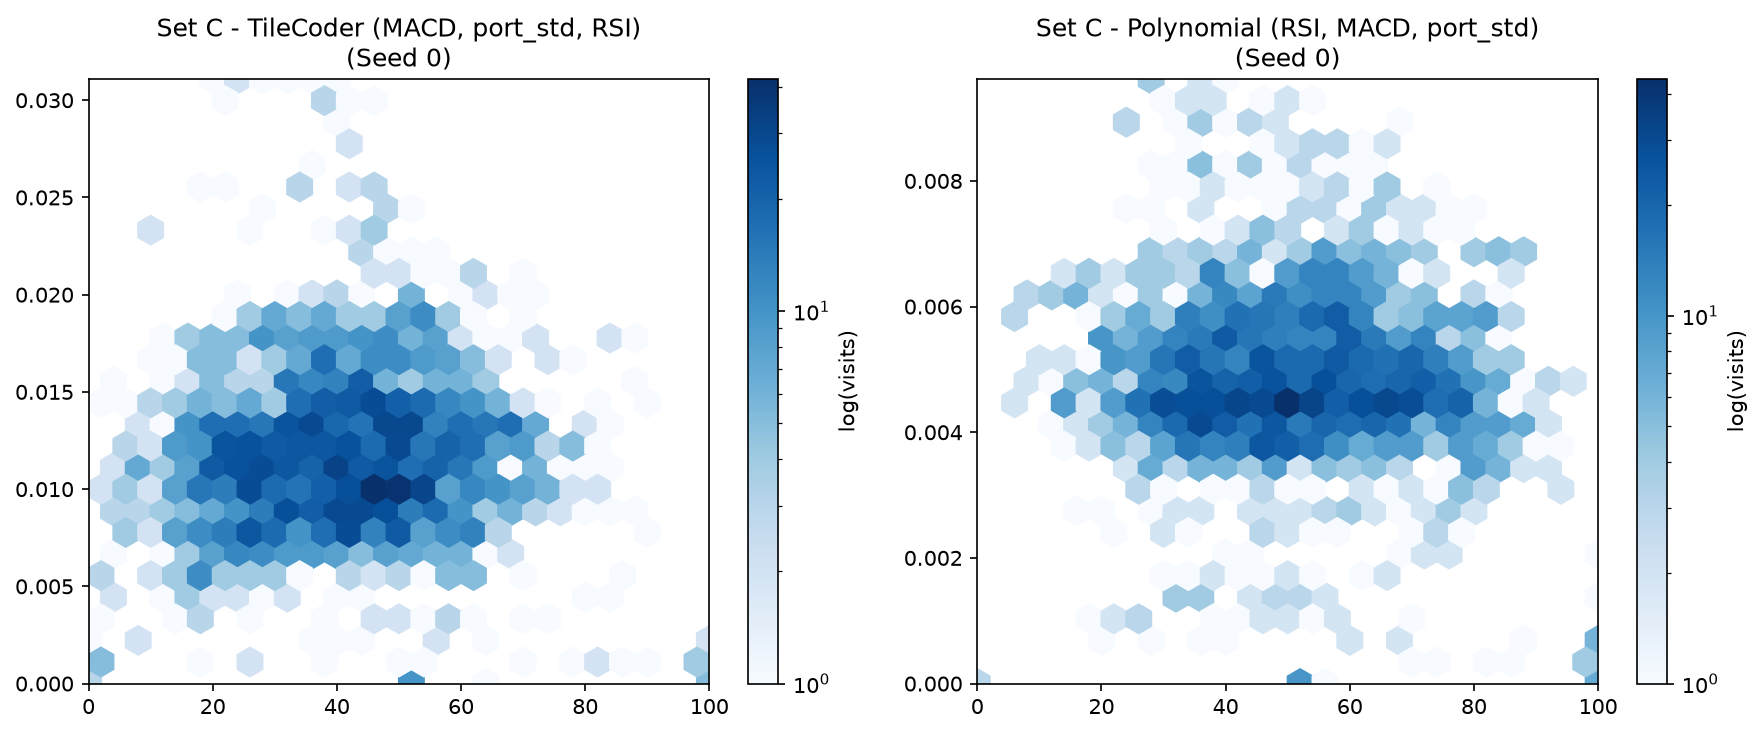
\includegraphics[width=0.9\textwidth]{charts/state_visit.png}
    \caption{State-visitation density (hexbin, log scale) over the RSI $\times$ volatility plane for the Set C agents (seed 0, 10 greedy episodes). Left: the tile-coded agent visits a broad region of the plane; right: the collapsed polynomial policy remains trapped in a narrow low-volatility band.}
     \label{fig:state_Visitation}
\end{figure}

Figure~\ref{fig:state_Visitation} shows the state-visitation density over 
the (MACD, Volatility, RSI) plane for the Set C agents, 
collected over 10 greedy episodes (2500 steps), 

Tile coding displays a diverse action distribution and the tile-coded agent 
explores the full volatility range (up to $0.03$), including the high-volatility crisis region. 

Correspondingly, the polynomial agent's visitation is confined to a narrow low-volatility 
band ($\mathrm{port\_std} \lesssim 0.009$), the region consistent with its single conservative allocation: 
since polynomial features generalize globally, no update can differentiate this region from the rest of the state space, 
and the policy never escapes it. 

Table~\ref{tab:top_actions} reports the five most frequent joint actions of every agent over the same rollouts. 

The most frequent actions also reveal the learned strategies: the best agent (Set A with Tiling) 
most often executes (2,0,0) --- buy BTC, sell bonds and ETF stocks --- i.e., rotation into the high-drift asset, 
whereas the allocation-based Set B agent alternates symmetric rebalancing actions ((2,1,2), (1,1,0), (0,1,0)), consistent with a static target-allocation policy.

\begin{table}[htbp]
  \centering
  \caption{Top 5 most used joint actions per agent (10 greedy episodes, seed 0, 2500 steps).}
  \label{tab:top_actions}
  \begin{tabular}{llrr}
    \toprule
    \textbf{Action ID} & \textbf{Description (Asset 0 / 1 / 2)} & \textbf{Count} & \textbf{\% of Total} \\
    \midrule
    \multicolumn{4}{l}{\textbf{Agent: Set A -- Raw (prices)}} \\
    (1, 1, 1) & Hold / Hold / Hold & 2,500 & 100.0\% \\
    \midrule
    \multicolumn{4}{l}{\textbf{Agent: Set A -- TileCoder (prices)}} \\
    (2, 0, 0) & Buy / Sell / Sell & 586 & 23.4\% \\
    (1, 2, 1) & Hold / Buy / Hold & 541 & 21.6\% \\
    (0, 1, 1) & Sell / Hold / Hold & 478 & 19.1\% \\
    (0, 1, 2) & Sell / Hold / Buy & 341 & 13.6\% \\
    (1, 0, 2) & Hold / Sell / Buy & 234 & 9.4\% \\
    \midrule
    \multicolumn{4}{l}{\textbf{Agent: Set B -- TileCoder (asset allocation)}} \\
    (2, 1, 2) & Buy / Hold / Buy & 862 & 34.5\% \\
    (1, 1, 0) & Hold / Hold / Sell & 715 & 28.6\% \\
    (0, 1, 0) & Sell / Hold / Sell & 578 & 23.1\% \\
    (2, 0, 2) & Buy / Sell / Buy & 105 & 4.2\% \\
    (0, 0, 1) & Sell / Sell / Hold & 74 & 3.0\% \\
    \midrule
    \multicolumn{4}{l}{\textbf{Agent: Set B -- Polynomial (asset allocation)}} \\
    (0, 2, 2) & Sell / Buy / Buy & 2,500 & 100.0\% \\
    \midrule
    \multicolumn{4}{l}{\textbf{Agent: Set C -- TileCoder (MACD, Volatility, RSI)}} \\
    (2, 0, 1) & Buy / Sell / Hold & 429 & 17.2\% \\
    (0, 2, 0) & Sell / Buy / Sell & 278 & 11.1\% \\
    (0, 2, 2) & Sell / Buy / Buy & 227 & 9.1\% \\
    (0, 0, 0) & Sell / Sell / Sell & 166 & 6.6\% \\
    (2, 1, 1) & Buy / Hold / Hold & 162 & 6.5\% \\
    \midrule
    \multicolumn{4}{l}{\textbf{Agent: Set C -- Polynomial (MACD, Volatility, RSI)}} \\
    (1, 2, 2) & Hold / Buy / Buy & 2,500 & 100.0\% \\
    \midrule
    \multicolumn{4}{l}{\textbf{Agent: Set C -- RBF (MACD, Volatility, RSI)}} \\
    (0, 2, 0) & Sell / Buy / Sell & 580 & 23.2\% \\
    (2, 0, 1) & Buy / Sell / Hold & 553 & 22.1\% \\
    (2, 2, 2) & Buy / Buy / Buy & 383 & 15.3\% \\
    (2, 0, 0) & Buy / Sell / Sell & 232 & 9.3\% \\
    (1, 1, 0) & Hold / Hold / Sell & 215 & 8.6\% \\
    \bottomrule
  \end{tabular}
\end{table}

\subsection{Greedy Rollout Example}
\begin{figure}[ht]
    \centering
    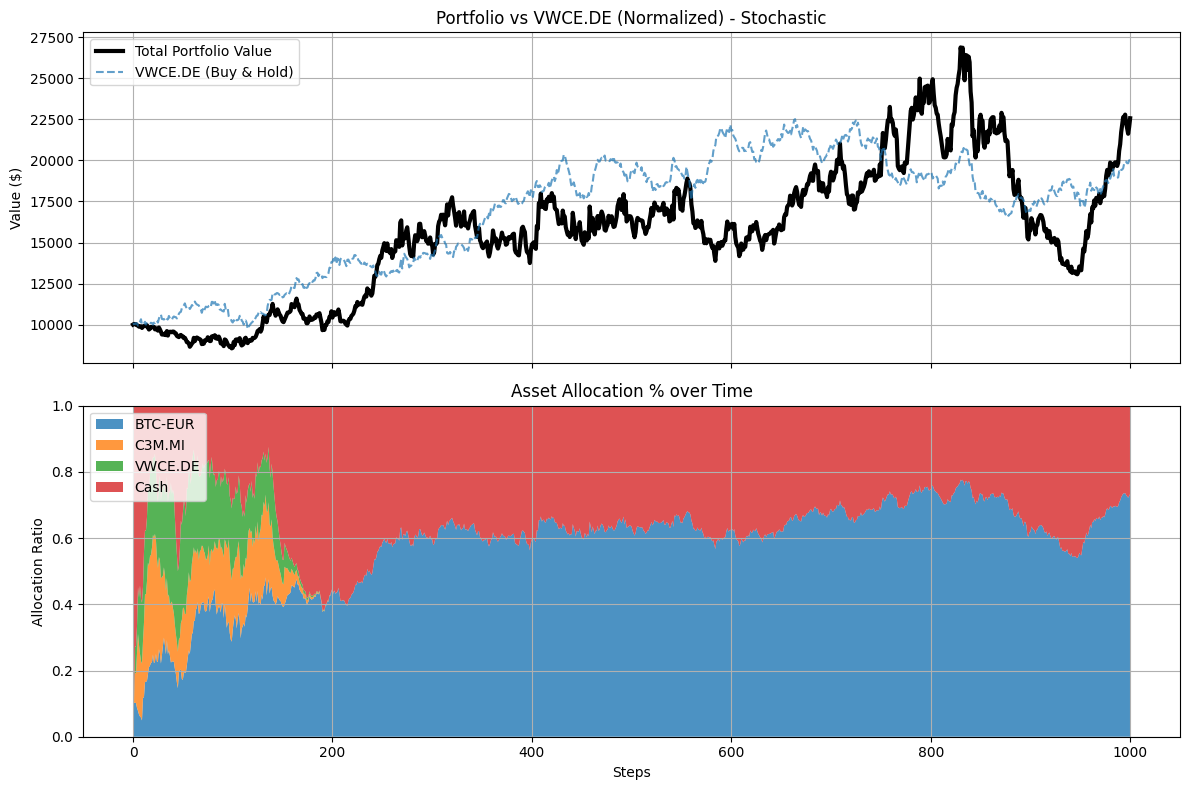
\includegraphics[width=0.9\textwidth]{charts/renderenv.png}
    \caption{Greedy rollout of the Set A with Tiling agent over 1000 steps (stochastic, regime-switching environment). Top: portfolio wealth vs.\ VWCE buy-and-hold benchmark. Bottom: allocation ratios over time.}
     \label{fig:renderenv}
\end{figure}

Figure~\ref{fig:renderenv} shows a single greedy rollout of the best-performing 
agent, Set A with Tiling, over $1000$ consecutive steps in the stochastic 
regime-switching environment with respect to VWCE buy-and-hold benchmark.

\section{Conclusion}

The experiments demonstrate that the feature map dictates the agent's success. 

Global approximations (like raw linear or polynomial features) fail drastically, either diverging numerically or collapsing into a degenerate, single-action policy. 

In contrast, local, sparse generalization via tile coding stabilizes semi-gradient SARSA and yields the best performance. 
RBF networks achieve similar returns but with significantly higher variance. 

Yet, even careful feature engineering cannot completely overcome the approximation-error floor of linear value-function approximation (VFA) in this noisy, regime-switching environment.

These results expose several structural limitations in the linear VFA framework. 

First, projection error is unavoidable: within-tile aliasing creates a representational 
hidden state that no amount of additional training can resolve. 
Second, stability is highly fragile, and global generalization often traps the agent in a feedback loop where it stops exploring. 

The linear framework is bottlenecked by the need for hand-crafted feature maps. 
As future work to bypass this projection-error floor is to experiment the transition to Deep Q-Networks (DQN \cite{mnih2015human}). 

\bibliography{references}

\end{document}